%==============================================================
%------------------JONATHAN TOBIAS DA SILVA--------------------
%---------------ENGENHARIA ELÉTRICA - 1ª TURMA-----------------
%-----------INSTITUTO FEDERAL - CAMPUS SERTÃOZINHO-------------
%--------------Main.tex, v1.0.0, JonathanTSilva----------------
%==============================================================

\documentclass[../Main.tex]{subfiles}

\newcommand*{\thead}[1]{\multicolumn{1}{|c|}{\bfseries #1}}
\newcommand{\x}[1]{\cellcolor{preto} #1}
\newcommand{\y}[1]{\cellcolor{cinza} #1}

\begin{document}
    Mencionar as etapas a serem realizadas até a conclusão do projeto.
    
    As Tabelas~\ref{tab:metas}~e~\ref{tab:cronograma} foram retiradas do projeto de iniciação científica "SILVA, J. T. da; DIAS, A. L.; TURCATO, A. C. \textbf{Sistema de diagnóstico para falhas em bombas hidráulicas por meio de análise de corrente elétrica e ferramentas de aprendizagem de máquinas}. p. 21, 2020"\ para auxiliar no desenvolvimento deste tópico.

    \begin{table}[H]
        \caption{Metas estabelecidas para a pesquisa.}
        \label{tab:metas}
        \centering
        \begin{tabular}{|>{\centering\arraybackslash}m{0.1\textwidth}|>{\raggedright\arraybackslash}m{0.9\textwidth}|}
            \hline
            \thead{METAS} & \thead{DESCRIÇÃO} \\
            \hline
            1 & Pesquisa bibliográfica \\
            \hline
            2 & Projeto e implementação da bancada experimental \\
            \hline
            3 & Implementação do sistema de automação para coleta de dados \\
            \hline
            4 & Realização de experimentos para coleta de dados \\
            \hline
            5 & Relatório Parcial entrega até 01/07/20 \\
            \hline
            6 & Desenvolvimento do sistema de diagnóstico \\
            \hline
            7 & Verificação de desempenho e validação dos resultados \\
            \hline
            8 & Gerar publicação científica em Congresso/Revista \\
            \hline
            9 & Relatório Final entrega até 30/11/2020 \\
            \hline
        \end{tabular}
    \end{table}
    
    \begin{table}[H]
        \centering
        \caption{Cronograma proposto para cumprimento das metas. }
        \label{tab:cronograma}
        \begin{tabular}{
        |>{\centering\arraybackslash}m{0.1\textwidth}
        |>{\centering\arraybackslash}m{0.075\textwidth}
        |>{\centering\arraybackslash}m{0.075\textwidth}
        |>{\centering\arraybackslash}m{0.075\textwidth}
        |>{\centering\arraybackslash}m{0.075\textwidth}
        |>{\centering\arraybackslash}m{0.075\textwidth}
        |>{\centering\arraybackslash}m{0.075\textwidth}
        |>{\centering\arraybackslash}m{0.075\textwidth}
        |>{\centering\arraybackslash}m{0.075\textwidth}
        |>{\centering\arraybackslash}m{0.075\textwidth}
        |}
            \hline
            \multicolumn{1}{|l|}{} & \multicolumn{9}{c|}{\textbf{MESES}}                 \\ \hline
            \thead{METAS}          & MAR & ABR & MAI & JUN & JUL & AGO & SET & OUT & NOV \\ \hline
            1                      & \y  & \y  & \y  & \y  & \x  & \x  & \x  & \x  &     \\ \hline
            2                      & \y  & \x  & \x  &     &     &     &     &     &     \\ \hline
            3                      &     & \y  & \y  & \x  & \x  &     &     &     &     \\ \hline
            4                      &     &     &     & \x  & \x  & \x  &     &     &     \\ \hline
            5                      &     &     & \y  & \y  &     &     &     &     &     \\ \hline
            6                      &     &     &     & \y  & \x  & \x  & \x  &     &     \\ \hline
            7                      &     &     &     &     &     & \x  & \x  &     &     \\ \hline
            8                      &     &     &     &     &     & \x  & \x  & \x  &     \\ \hline
            9                      &     &     &     &     &     &     & \x  & \x  & \x  \\ \hline
        \end{tabular}
        \begin{flushleft}
            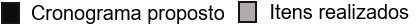
\includegraphics[scale=0.7]{Images/leg1.jpg}
        \end{flushleft}
    \end{table}
\end{document}